\documentclass[handout]{beamer}
\usepackage{graphicx}
\graphicspath{ {./} }
% \usetheme{Berkeley}
\title{An Experimentation Toolkit for Robotics Control and Manipulation Tasks using Reinforcement Learning Algorithms}
\subtitle{A Robot Learning Gym}
\author{Ashwin Reddy, The Harker School}
\date % (optional)
{March 23, 2017}

\begin{document}
\frame{\titlepage}
\begin{frame}
    \frametitle{Introduction}
    \begin{figure}
        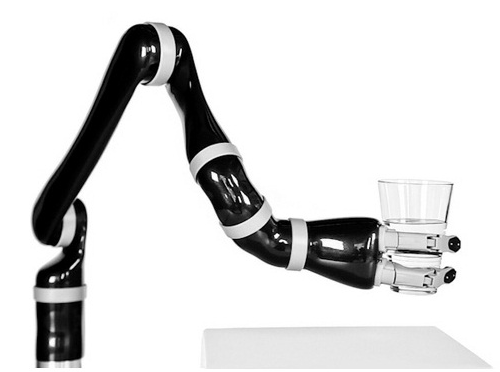
\includegraphics[scale=0.2]{arm}
        \caption{A robot arm}
    \end{figure}
    \begin{itemize}
        \item{Suppose we have the robot pictured above}
        \item{How to manipulate objects in the real world autonomously?}
        \item{Maybe use AI? However, not many tools for AI-based robotics}
        \item{To develop smart robots, a good toolkit is required}
    \end{itemize}
\end{frame}
\begin{frame}
    \frametitle{Purpose}
    \begin{itemize}
        \item{Build a toolkit for prototyping AI-based robotics control algorithms}
        \item{Requirements}
        \begin{itemize}
            \item{Should be able to test code quickly and often}
            \item{Use a fast simulator}
            \item{Easy to get started (minimal setup barriers)}
            \item{Visualization tools}
        \end{itemize}
        \item{Try to use popular tools}
    \end{itemize}
\end{frame}

% \begin{frame}
%     \frametitle{Background: Reinforcement Learning / Machine Learning (Neural Networks)}
%     \begin{itemize}
%         \item{
%         \begin{figure}[p]
%             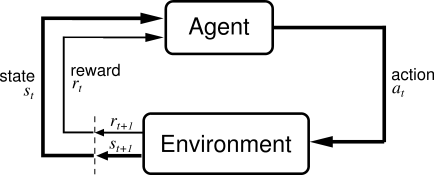
\includegraphics[scale=0.25]{diagram1}
%         \end{figure}}
%         \item{How can we train the agent to pick actions to maximize reward?}
%         \begin{figure}[p]
%             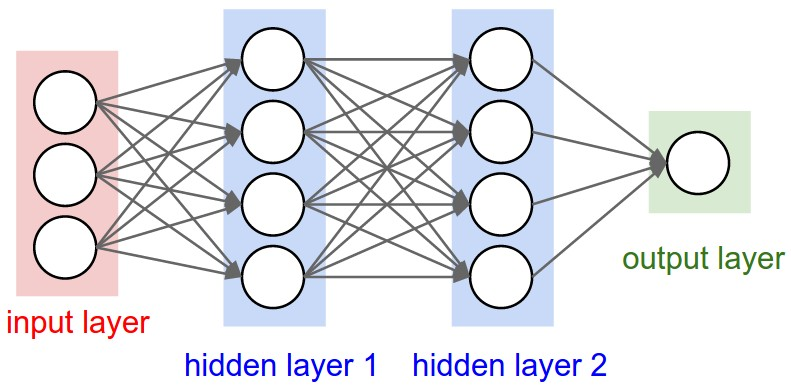
\includegraphics[scale=0.2]{diagram2}
%         \end{figure}
%         \item{Goal: make predictions}
%         \item{Given many samples of $(x,f(x))$, learn $h_\theta(x)\approx{f(x)}$}
%     \end{itemize}
% \end{frame}
% \begin{frame}
%     \frametitle{What makes Deep RL for Robotics hard?}
%     \begin{itemize}
%         \item{Algorithms}
%         \begin{itemize}
%             \item{Lack of large datasets (i.e: poor supervision)}
%             \item{Curse of dimensionality}
%             \item{Sparse time-delayed rewards}
%             \item{Exploration vs. Exploitation}
%             \item{Continuous control harder than discretized actions}
%         \end{itemize}
%         \item{Noisy input, unreliable outputs}
%         \item{Visual Occlusions}
%         \item{Running on a real robot is expensive}
%     \end{itemize}
% \end{frame}
\begin{frame}
    \frametitle{Current Tools}
    \begin{itemize}
        \item{OpenAI Gym: mini-games for testing algorithms}
    \end{itemize}
    \begin{figure}
        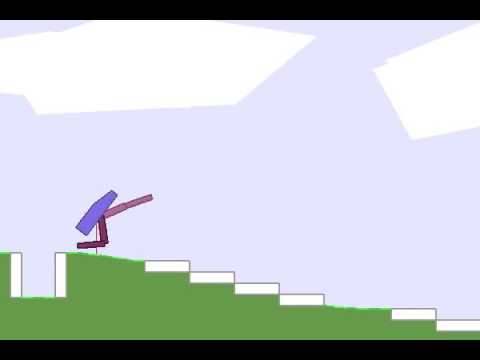
\includegraphics[scale=0.2]{walker}
        \caption{Bipedal walking in Gym}
    \end{figure}
    \begin{itemize}
        % \item{OpenAI RL Lab implements some common RL algorithms}
        % \item{Guided Policy Search: package for an algorithm of the same name}
        % \item{DeepMind's Lab: tests RL algorithms with 3D first-person games}
        \item{TensorFlow: library for machine learning (AI)}
        \item{MuJoCo: 3D physics simulator}
        \item{These are 3 main projects used in the toolkit}
    \end{itemize}
\end{frame}
\begin{frame}
    \frametitle{Designing the Framework}
    \begin{itemize}
        \item{Plan}
        \begin{itemize}
            \item{Investigate current tools (pros/cons)}
            \item{Build a core framework to plug above tools into}
            \item{Extend OpenAI Gym package}
            \item{Collect robot "models" for MuJoCo}
            \item{Implement some algorithms}
        \end{itemize}
    \end{itemize}
\end{frame}
\begin{frame}
    \frametitle{Designing the Framework: Process}
    \begin{itemize}
        \item{Attempted mixed robots and environments}
        \item{Learn and incorporate TensorFlow}
        \item{Open source code and publish online (GitHub)}
    \end{itemize}
\end{frame}
\begin{frame}
    \frametitle{Results}
    \begin{itemize}
        \item{One possible use case might be benchmarking different algorithms}
    \end{itemize}
    \begin{figure}
        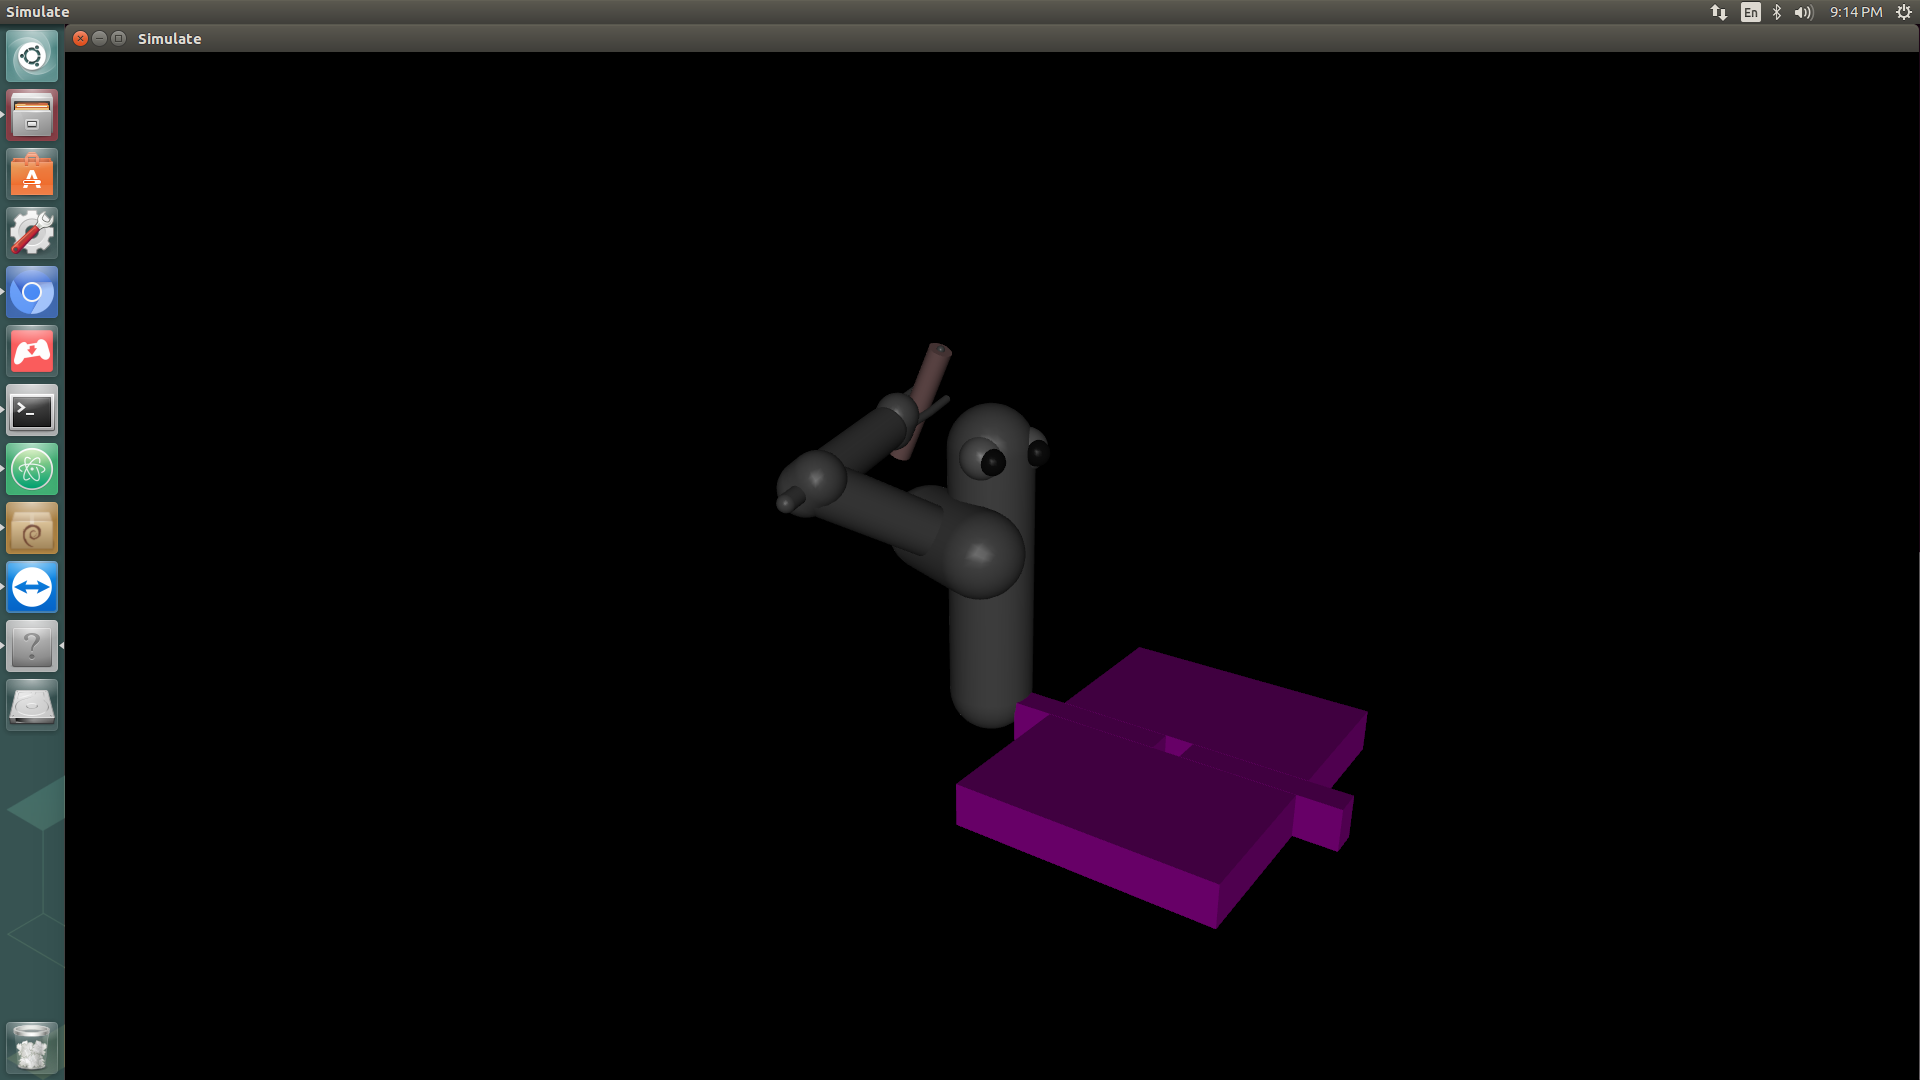
\includegraphics[scale=0.1]{sim1}
        \caption{Peg Insertion Task in MuJoCo}
    \end{figure}
\end{frame}
\begin{frame}
    \frametitle{Visualizations}
    \begin{figure}
        \centering
        \begin{minipage}{0.45\textwidth}
            \centering
            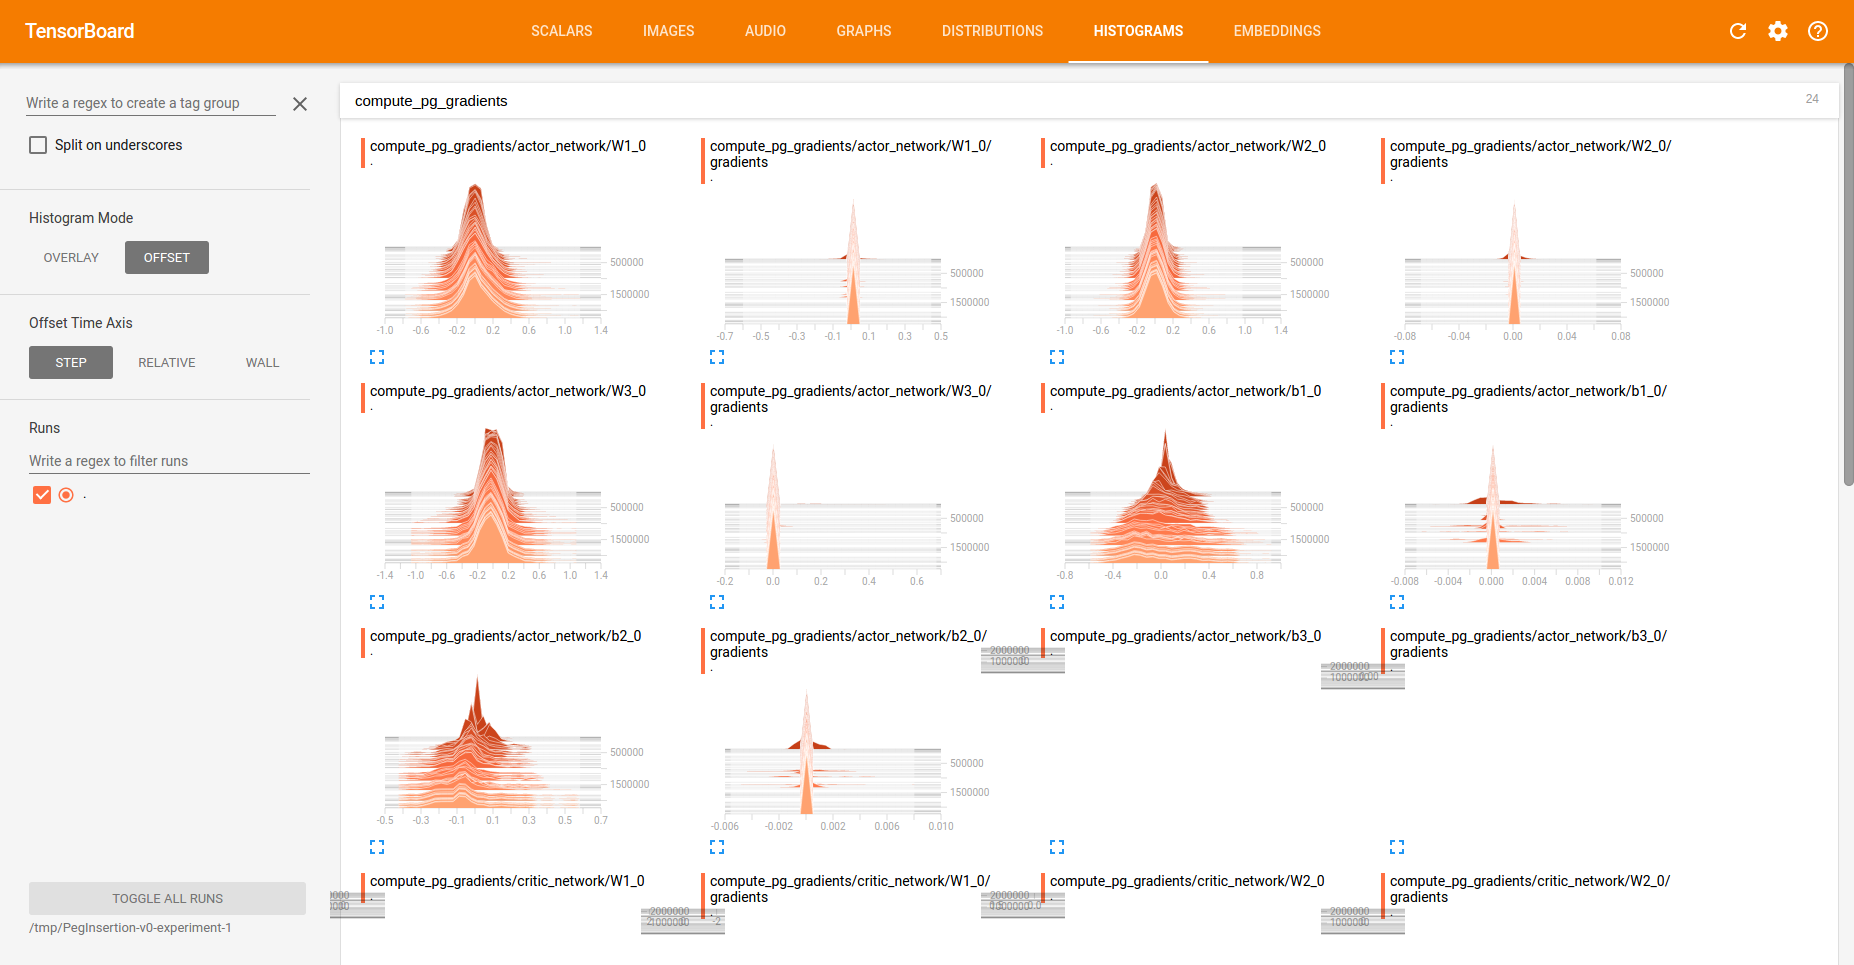
\includegraphics[width=0.9\textwidth]{ex1} % first figure itself
            \caption{TensorFlow's histograms}
            \end{minipage}\hfill
            \begin{minipage}{0.45\textwidth}
                \centering
                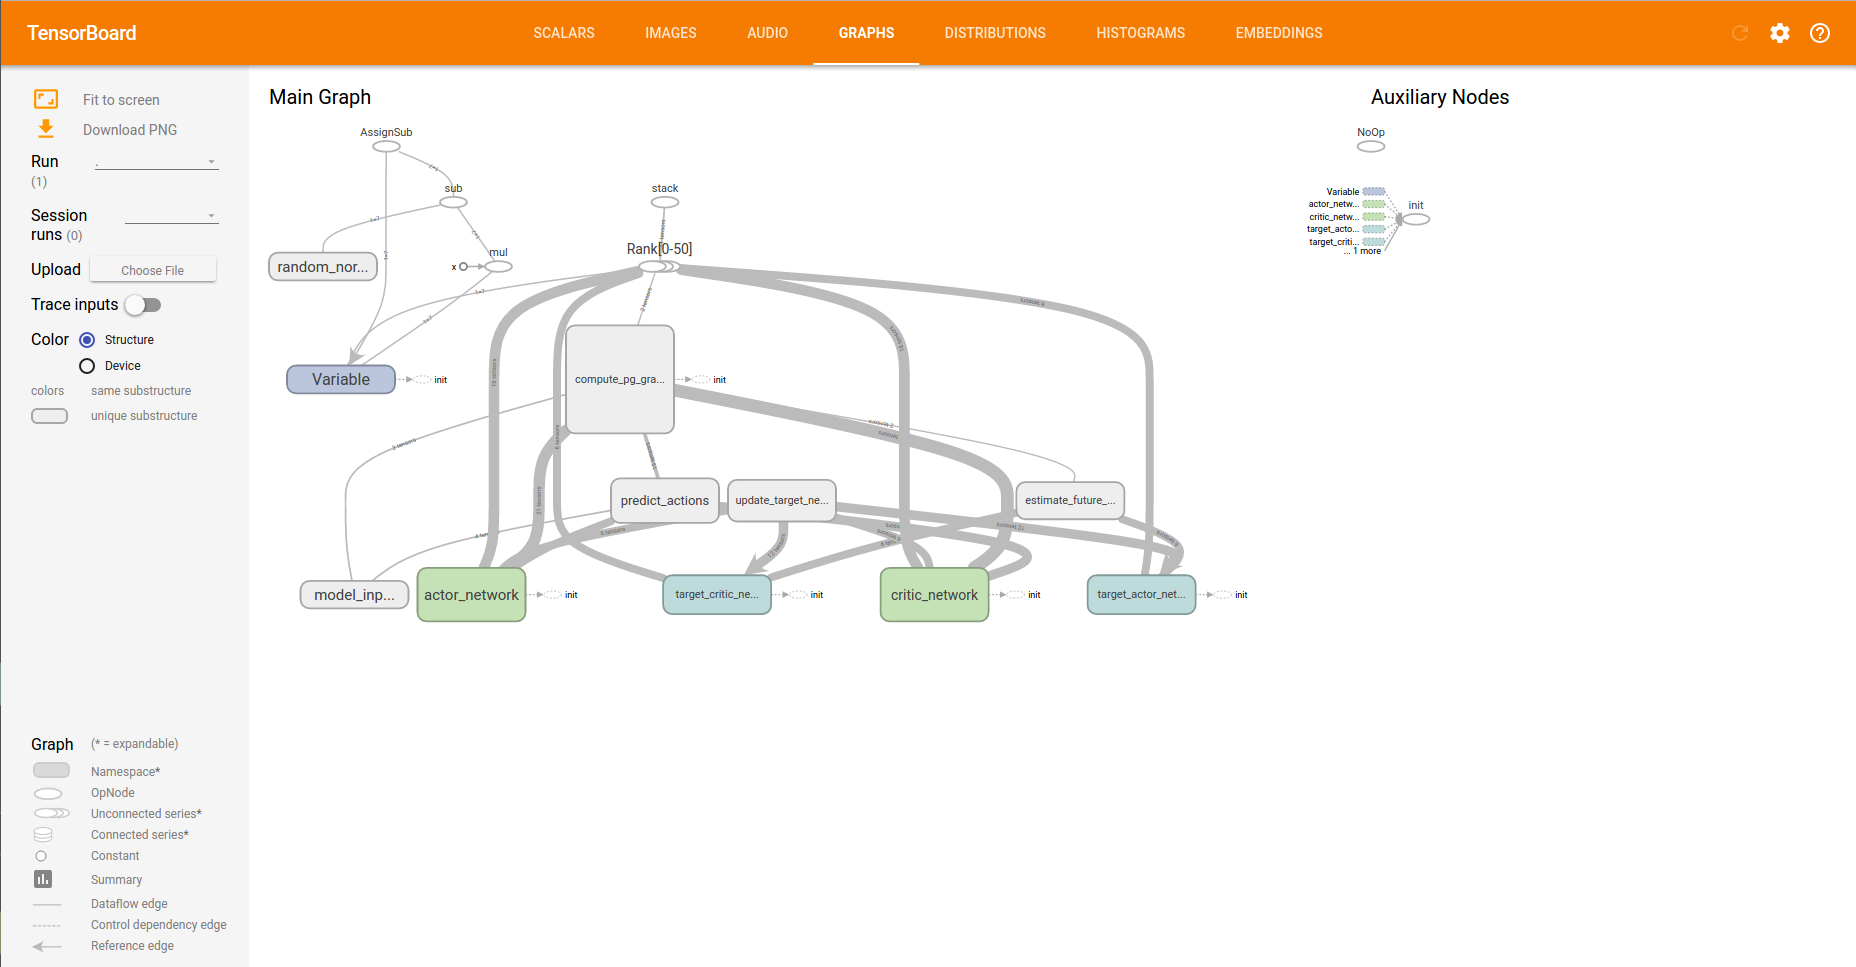
\includegraphics[width=0.9\textwidth]{ex2} % second figure itself
                \caption{TensorFlow's visual network architecture}
            \end{minipage}
        \end{figure}
        \begin{figure}
            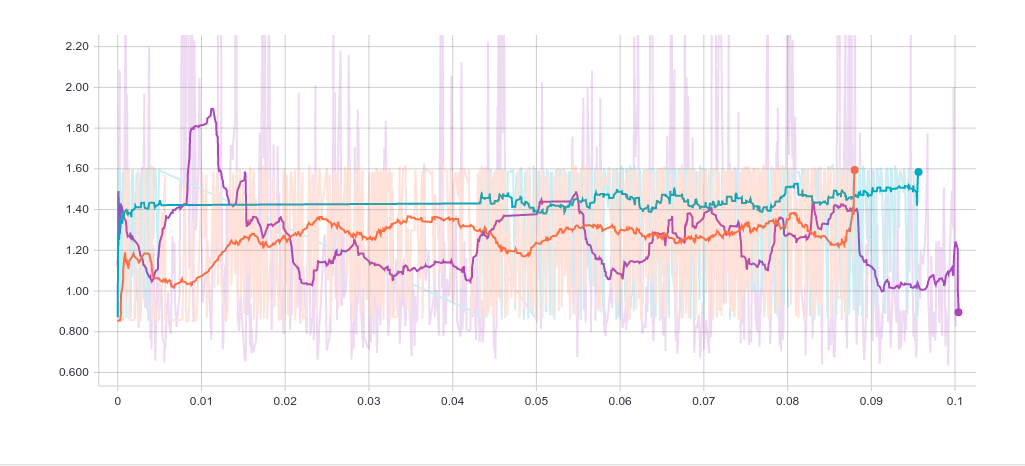
\includegraphics[scale=0.1]{smoothed}
            \caption{Reward vs. time graph for a few algorithms}
        \end{figure}
    \end{frame}
    \begin{frame}
        \frametitle{Conclusion}
        \begin{itemize}
            \item{Made it easier for myself and others to try new ideas quickly}
            \item{Future Work}
            \begin{itemize}
                \item{Maintain the framework and create more extensive documentation}
                \item{Experiment with other network architectures}
                \item{Benchmark more deep learning based algorithms}
                \item{Include more environments/tasks/robots}
            \end{itemize}
        \end{itemize}
    \end{frame}
    \begin{frame}
        \frametitle{Acknowledgements / References}
        \begin{itemize}
            \item{Thanks to}
            \begin{itemize}
                \item{Mr. Martin Baynes for sponsoring this project}
                \item{Soroush Nasiriany, an undergraduate researcher at UC Berkeley, and}
                \item{Abhishek Gupta, a PhD student at UC Berkeley for feedback on this project}
            \end{itemize}
        \end{itemize}
    \end{frame}
    \end{document}
